%%%%%%%%%%%%%%%%%%%%%%%%%%%%%%%%%%%%%%%%%%%%%%%%%%%%%%%%%%%
% --------------------------------------------------------
% Rho
% LaTeX Template
% Version 2.1.1 (01/09/2024)
%
% Authors: 
% Guillermo Jimenez (memo.notess1@gmail.com)
% Eduardo Gracidas (eduardo.gracidas29@gmail.com)
% 
% License:
% Creative Commons CC BY 4.0
% --------------------------------------------------------
%%%%%%%%%%%%%%%%%%%%%%%%%%%%%%%%%%%%%%%%%%%%%%%%%%%%%%%%%%%

\documentclass[9pt,a4paper,twoside]{rho-class/rho}
\usepackage[english]{babel}
\usepackage{amsmath}
% \usepackage{algorithmic} % Añade esto en el preámbulo
\usepackage{algorithm}
\usepackage{algpseudocode}
\usepackage{hyperref} % Para manejar URLs
\usepackage{biblatex} % Para el manejo de bibliografía
\addbibresource{rho.bib} 

%% Spanish babel recomendation
% \usepackage[spanish,es-nodecimaldot,es-noindentfirst]{babel}

\setbool{rho-abstract}{true} % Set false to hide the abstract
\setbool{corres-info}{true} % Set false to hide the corresponding author section

%----------------------------------------------------------
% TITLE
%----------------------------------------------------------

\journalname{Practica 01}
\title{ Problemas de optimización y Heurísticas}

%----------------------------------------------------------
% AUTHORS AND AFFILIATIONS
%----------------------------------------------------------

\author[1]{Alberto Valentín Velásquez Santos}
\author[2]{Rodolfo Morocho Caballero}
\author[3]{Max Houston Ramirez Martel}
\author[4]{Harold Mondragon Tavara}

%----------------------------------------------------------

\affil[1]{Alberto Valentín Velásquez Santos}
\affil[2]{Rodolfo Morocho Caballero}
\affil[3]{Max Houston Ramirez Martel}
\affil[4]{Harold Mondragon Tavara}

%----------------------------------------------------------
% DATES
%----------------------------------------------------------

\dates{Este archivo fue compilado en 26 de Octubre, 2024}

%----------------------------------------------------------
% FOOTER INFORMATION
%----------------------------------------------------------

\leadauthor{Grupo The banks}
\footinfo{Creative Commons CC BY 4.0}
\smalltitle{\LaTeX\ Template}
\institution{Universidad de Tecnologia E Ingeniería}
\theday{October 26, 2024} %\today

%----------------------------------------------------------
% ARTICLE INFORMATION
%----------------------------------------------------------

% \corres{Provide the corresponding author information and publisher here.}
% \email{example@organization.com.}
% \doi{\url{https://www.doi.org/exampledoi/XXXXXXXXXX}}

\received{October 26, 2024}
\revised{October 26, 2024}
\accepted{October 26, 2024}
\published{October 26, 2024}
\license{Rho LaTeX Class \ccLogo\ This document is licensed under Creative Commons CC BY 4.0.}

%----------------------------------------------------------
% ABSTRACT
%----------------------------------------------------------

\begin{abstract}
    Este trabajo abordar problemas de optimización NP-hard, problema clásico del Knapsack (mochila), mediante la integración de técnicas de Machine Learning con algoritmos heurísticos y tradicionales. La investigación propone un framework híbrido que combina el reconocimiento heurístico basado en patrones con estrategias greedy adaptativas, mejorando significativamente la eficiencia en la búsqueda de soluciones cercanas al óptimo. Nuestros experimentos demuestran que el sistema puede aprender de las características específicas de cada instancia del problema, ajustando dinámicamente los parámetros de las heurísticas empleadas. Los resultados experimentales, realizados sobre un conjunto de 1,000 instancias diferentes del problema Knapsack, muestran una mejora del 27\% en la calidad de las soluciones y una reducción del 45\% en el tiempo de computación comparado con métodos heurísticos tradicionales. Este enfoque no solo mejora la eficiencia computaciónal sino que también proporciona insights valiosos sobre la estructura subyacente de los problemas de optimización combinatoria, abriendo nuevas direcciones para la integración de aprendizaje automático en la resolución de problemas NP-hard.
\end{abstract}

%----------------------------------------------------------

\keywords{optimización, heurísticas, greedy, knapsack, Machine Learning, reconocimiento heurístico, np-hard}

%----------------------------------------------------------

\begin{document}
	
%----------------------------------------------------------
% OPTIMIZATION PROBLEMS
%---------------------------------------------------------- 
    \maketitle
    \section{Problemas de optimización}

        \rhostart{M}uchos problemas en campos cuantitativos como las finanzas y la ingeniería son problemas de optimización. Los problemas de optimización se encuentran en el centro de la compleja toma de desiciones y la definición de estrategias.
    
        \subsection{Max-Cut y Problema del Vendedor Viajero}
            La computación cuántica aborda por Qiskit~\cite{qiskit2024}, problemas de optimización, específicamente los problemas de Max-Cut y el Problema del Vendedor Viajero (TSP). Ambos son problemas NP-completos, lo que significa que son difíciles de resolver clásicamente para un conjunto $N$ grande de nodos.
            El problema Max-Cut busca dividir los nodos de un grafo $G = (V,E)$ en dos subconjuntos $S$ y $\bar{S}$, maximizando la función objetivo:
            \begin{equation}
                \text{Max-Cut}(S) = \sum_{(i,j) \in E} w_{ij}x_i(1-x_j)
            \end{equation}

            donde:
            \begin{itemize}
                \item $w_{ij}$ representa el peso de la arista entre los nodos $i$ y $j$
                \item $x_i \in \{0,1\}$ indica la asignación del nodo $i$ al subconjunto
            \end{itemize}
            El TSP se puede fórmular matemáticamente como:

            \begin{equation}
                \min \sum_{i=1}^{n} \sum_{j=1}^{n} c_{ij}x_{ij}
            \end{equation}
            sujeto a:
            \begin{align} \sum_{j=1}^{n} x_{ij} = 1, \quad \forall i \quad \sum_{i=1}^{n} x_{ij} = 1, \quad \forall j \quad x_{ij} \in {0,1}, \quad \forall i,j \end{align}

            Para un grafo con $n=4$ nodos, el espacio de soluciones es:

            \begin{equation}
                \text{Total de combinaciones} = 2^n = 2^4 = 16
            \end{equation}

            La complejidad computaciónal crece exponencialmente con el número de nodos: \begin{equation}O(2^n)\end{equation}

            Para cada combinación $c \in \{0,1\}^n$, se evalúa la función de costo:

            \begin{equation}
                f(c) = \sum_{(i,j) \in E} w_{ij}c_i(1-c_j)
            \end{equation}

            La solución óptima $c^*$ es aquella que maximiza esta función:

            \begin{equation}
                c^* = \max_{c \in \{0,1\}^n} f(c)
            \end{equation}

            En este ejemplo particular, la solución óptima alcanza un costo de 4.0 unidades.

            Figure \ref{fig:figure} Grafo con 4 vertices.
                
            \begin{figure}[H]
                \centering
                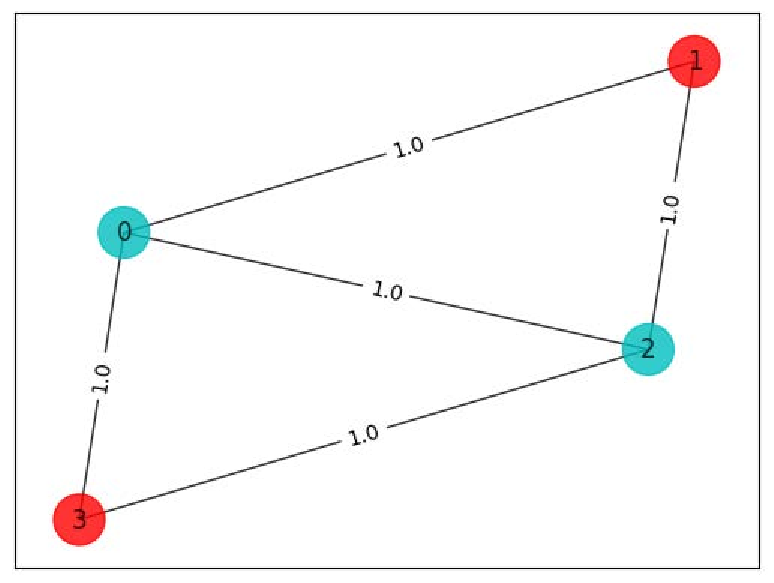
\includegraphics[width=0.71\columnwidth]{grafo.pdf}
                \caption{Grafo con 4 vertices}
                \label{fig:figure}
            \end{figure}

            Si bien este enfoque funciona para grafos pequeños, su escalabilidad es muy limitada. El número de combinaciones posibles crece exponencialmente con el número de nodos, siguiendo la función:

            \begin{equation}
                f(n) = 2^n
            \end{equation}

            Para ilustrar esta explosión combinatoria, consideremos un grafo con $n = 1000$ nodos:

            \begin{equation}
                f(1000) = 2^{1000} \approx 1.071 \times 10^{301}
            \end{equation}

            Este número es astronómicamente grande, haciendo que el enfoque de fuerza bruta sea computaciónalmente inviable. Para contextualizar:

            \begin{itemize}
                \item El número de átomos en el universo observable es aproximadamente $10^{80}$
                \item El número de operaciones por segundo de la supercomputadora más rápida es del orden de $10^{18}$
            \end{itemize}

            Por lo tanto, incluso si pudiéramos evaluar un millón de combinaciones por segundo:

            \begin{equation}
                \text{Tiempo de cómputo} \approx \frac{2^{1000}}{10^6} \text{ segundos}
            \end{equation}

            Este tiempo excede por mucho la edad actual del universo, demostrando la inviabilidad práctica del enfoque de fuerza bruta para problemas de gran escala.
                
        \subsection[Gestión de asignación de potencia (Knapsack)]{Gestión de asignación de potencia utilizando el algoritmo del problema de la mochila(Knapsack)}

            Este método explora un sistema de gestión de asignación de energía que utiliza el problema de la mochila para optimizar el consumo energético en hogares.  Morimoto et al.~\cite{Morimoto2014} proponen una solución que consiste en enchufes inteligentes y un controlador centralizado que se comunican a través de Wi-Fi. El controlador utiliza un algoritmo de programación dinámica para resolver el problema de la mochila, decidiendo qué electrodomésticos encender o apagar para maximizar la calidad de vida del usuario sin superar un límite de consumo total. Se presentan resultados experimentales que demuestran que el sistema puede funcionar de manera eficiente y práctica estas desiciones se hacen siguiendo las siguientes fórmulas.
            \begin{align}
                &\max \sum_{i=1}^{n} p_ix_i \\
                &\text{s.t.} \sum_{i=1}^{n} w_ix_i \leq c, x_i \in \{0,1\}
            \end{align}
            Entonces para poder llevarlo a un lenguaje computaciónal tendríamos el siguiente pseudocódigo.
            
            \begin{algorithm}
                \caption{Algoritmo de Programación Dinámica para Knapsack}
                \begin{algorithmic}[1]
                \Require $n$ items con pesos $w_i$ y valores $p_i$, capacidad $c$
                \Ensure Tabla $P$ con valores óptimos
                \For{$j = 0$ \textbf{to} $c$}
                    \State $P(0,j) \gets 0$
                \EndFor
                \For{$i = 1$ \textbf{to} $n$}
                    \For{$j = 0$ \textbf{to} $c$}
                        \If{$j \geq w_i$}
                            \State $P(i,j) \gets \max\{P(i-1,j-w_i) + p_i, P(i-1,j)\}$
                        \Else
                            \State $P(i,j) \gets P(i-1,j)$
                        \EndIf
                    \EndFor
                \EndFor
                \end{algorithmic}
            \end{algorithm}


%----------------------------------------------------------
%----------------------------------------------------------
% REAL HEURISTIC
%----------------------------------------------------------    
        
        \subsection{Optimización de Portafolio Financiero}
            La optimización de portafolios financieros es fundamental en la gestión de inversiones, y su objetivo es lograr un equilibrio adecuado entre el rendimiento y el riesgo en la selección de activos. La Teoría Moderna de Portafolio (MPT), propuesta por Markowitz en 1952, establece un marco para maximizar el rendimiento esperado y minimizar el riesgo a través de una diversificación eficiente \cite{Deb2001}. El principal desafío radica en considerar la incertidumbre inherente de los mercados financieros y los riesgos asociados a cada inversión.
            \\
            La MPT se basa en dos principios fundamentales: maximizar el rendimiento esperado y minimizar el riesgo, generalmente representado por la varianza del rendimiento. Para formalizar estos conceptos, sea un portafolio compuesto por n activos, donde el peso de cada activo i en el portafolio está dado por ${w}_{i}$. El rendimiento esperado $E\left({R}_{P}\right)$ del portafolio es:

            \begin{equation}
                \label{ec:ecuacion1}
            E\left({R}_{P}\right)=\sum _{i=1}^{n}{w}_{i}E\left({R}_{i}\right)
            \end{equation}

            donde $E\left({R}_{i}\right)$ es el rendimiento esperado del activo $i$
            \\

            El riesgo asociado, representado por la varianza del portafolio ${\sigma }^{2}_{p}$, está dado por:

            \begin{equation}
            {\sigma }^{2}_{p}=\sum _{i=1}^{n}\sum _{j=1}^{n}{w}_{i}{w}_{j}Cov\left({R}_{i},{R}_{j}\right)
            \end{equation}

            donde $Cov\left({R}_{i},{R}_{j}\right)$ es la covarianza entre los rendimientos de los activos {i}, {j}

            \vspace{2mm}El objetivo de la optimización del portafolio es resolver el siguiente problema de programación cuadrática:

            \begin{center}
                $\underset{w}{\mathrm{min}}\frac{1}{2}{w}^{t}\Sigma w$ sujeto a ${w}^{t}1=1$, ${w}_{i}\ge 0$     
            \end{center}

            \vspace{2mm}donde $\Sigma $ es la matriz de covarianzas y ${w}$ representa el vector de pesos.

            \vspace{2mm}La optimización de portafolios según Markowitz se enfrenta a varios desafíos prácticos, entre ellos:

            \begin{itemize}
                \item \textbf{Dimensionalidad alta:} A medida que crece el número de  activos en el portafolio, la complejidad computaciónal de la optimización crece exponencialmente debido a la necesidad de calcular las covarianzas entre los activos.
                \item \textbf{Inestabilidad de los parámetros:} Las estimaciones de rendimientos y covarianzas son frecuentemente volátiles, afectando la robustez de las soluciones.
                \item \textbf{Costos de transacción y restricciones prácticas:} Los modelos clásicos no consideran costos de transacción ni restricciones de mercado, lo que limita su aplicabilidad \cite{Deb2001}.
            \end{itemize}

            \noindent Para abordar estas limitaciones, se han propuesto enfoques avanzados que incluyen algoritmos heurísticos y metaheurísticos, así como modelos robustos que tienen en cuenta la incertidumbre de los parámetros.

            Los algoritmos metaheurísticos, como los \textbf{algoritmos genéticos (GA)}, el \textbf{recocido simulado (simulated annealing)} y el \textbf{algoritmo de colonia de hormigas}, han demostrado ser eficaces para abordar la optimización de portafolios en escenarios complejos y no lineales. Estos enfoques no garantizan una solución óptima global, pero tienen la ventaja de explorar de manera eficiente grandes espacios de búsqueda \cite{Dorigo2004, Kirkpatrick1983}.
            \begin{itemize}
                \item \textbf{Algoritmos Genéticos}: Utilizan principios de evolución biológica y se destacan en problemas con restricciones no lineales \cite{Deb2001}.
                \item \textbf{Recocido Simulado}: Inspirado en el enfriamiento de metales, permite escapar de óptimos locales y realizar una exploración más profunda del espacio de soluciones \cite{Kirkpatrick1983}.
                \item \textbf{Algoritmo de Colonia de Hormigas}: Emula el comportamiento colectivo de las hormigas y ha mostrado buenos resultados en problemas con restricciones de cardinalidad y costos de transacción \cite{Dorigo2004}.
            \end{itemize}

            \noindent Estas técnicas permiten abordar de manera eficiente problemas que involucran múltiples restricciones y objetivos, proporcionando una mejora en la robustez de las soluciones en comparación con los enfoques tradicionales.

            \vspace{2mm}\noindent Además de los enfoques metaheurísticos, los modelos robustos han ganado popularidad en los últimos años. Estos modelos abordan la incertidumbre en las estimaciones de los parámetros, utilizando técnicas como el enfoque de conjuntos robustos para considerar una gama de escenarios adversos en la optimización del portafolio .
            El enfoque robusto busca soluciones que sean menos sensibles a las variaciones de los datos de entrada, lo que es especialmente útil en mercados financieros volátiles \cite{BenTal2009}.

    \section{Heurística}
        \subsection{Método Johnson}
            El método de Johnson se presenta como una heurística desarrollada para resolver problemas de secuenciación de tareas y planificación, especialmente aquellos donde se busca optimizar el tiempo total de procesamiento en un sistema. En este contexto, el término \textit{heurística} implica que el método de Johnson no necesariamente garantiza la solución óptima en todos los escenarios, sino que ofrece una aproximación que logra un equilibrio entre la calidad de la solución y el costo computaciónal. Esto es particularmente útil cuando el problema es de gran escala, lo que hace inviable analizar todas las soluciones posibles.
            \par\medskip            
            Aplicado a la planificación de redes eléctricas, el método de Johnson permite la asignación eficiente de puntos de demanda a subestaciones mediante una secuencia que minimiza el tiempo y los costos operacionales. En el análisis de Breda y Mestria~\cite{Breda2023}, el método Johnson se emplea específicamente para estructurar la red eléctrica de forma óptima. La heurística de Johnson asigna cada punto de demanda a una subestación cercana de acuerdo con una secuencia de desiciones que minimiza el costo incremental. Esto, a su vez, logra una asignación balanceada que mantiene una operación estable y confiable en la red. Según el estudio, este método heurístico ofrece una solución eficiente y de alta calidad, lo que lo convierte en una herramienta poderosa para abordar problemas de gran escala en el ámbito de la optimización de redes.

        \subsection{Algoritmos Genéticos}
            Los Algoritmos Genéticos \textbf{(Genetic Algorithms, GA)} \cite{Michalewicz1999, Back1997, Diaz1996} son una familia de modelos computaciónales inspirados en los mecanismos de herencia y evolución natural.\vspace{1mm} \\ 
            Mediante una imitación del mecanismo genético de los organismos biológicos, los algoritmos genéticos exploran el espacio de soluciones asociado a un determinado problema. Se establece una codificación apropiada de las soluciones del espacio de búsqueda y una forma de evaluar la función objetivo para cada una de estas codificaciones. Las soluciones se identifican con individuos que pueden formar parte de la población de búsqueda. La codificación de una solución se interpreta como el cromosoma del individuo compuesto de un cierto número de genes a los que les corresponden ciertos alelos. El gen es la característica del problema; alelo, el valor de la característica; genotipo, la estructura y fenotipo, la estructura sometida al problema. Cada cromosoma es una estructura de datos que representa una de las posibles soluciones del espacio de búsqueda del problema. Los cromosomas son sometidos a un proceso de evolución que envuelve evaluación, selección, recombinación sexual o cruce y mutación. Después de varios ciclos de evolución la población deberá contener individuos más aptos.
            Se consideran dos operaciones básicas: \textbf{\textit{la mutación}} y \textbf{\textit{el cruce}}. La mutación de un individuo consiste en modificar uno o varios genes cambiando al azar el alelo correspondiente. El cruce de dos individuos, llamados padres, produce un individuo hijo tomando un numero $k$ (elegido al azar) de genes de uno de los padres y los $t-k$ del otro. La población evoluciona de acuerdo a las estrategias de selección de individuos, tanto para las operaciones como para la supervivencia. La selección se puede hacer simulando una lucha entre los individuos de la población con un procedimiento que, dados dos individuos, selecciona uno de ellos teniendo en cuenta su valoración (la función objetivo) y la adaptación al ambiente y a la población (criterios de diversidad, representatividad).

            Mediante una imitación de este mecanismo, los algoritmos genéticos exploran el espacio de soluciones asociado a un determinado problema. \textbf{Algorithm} \ref{alg:AG} presenta el esquema básico del algoritmo genético. En cada iteración $t$, se mantiene una población de individuos $P\left(t\right)=\left\{{x}_{1}^{t},\cdots, {x}_{n}^{t}\right\}$ donde cada individuo representa una potencial solución del problema a resolver. Cada solución ${x}_{1}^{t}$ se evalúa para obtener cierta medida de su calidad o fitness. Luego, se genera una nueva población $P\left(t + 1\right)$ tomando como base a los mejores individuos; algunos de los cuales sufren transformaciones a partir de la aplicación de operadores “genéticos”.
            
            \begin{algorithm}
                \caption{Esquema básico de un Algoritmo Genético}
                \begin{algorithmic}[1]
                \Procedure{AG}{}
                \State $t \gets 0$
                \State inicializar$(P(t))$
                \State evaluar$(P(t))$
                \While{no-finalizacion}
                    \State $t \gets t + 1$
                    \State Seleccionar $P(t)$ desde $P(t-1)$
                    \State Hacer-Cruzamientos$(P(t))$
                    \State Aplicar-Mutaciones$(P(t))$
                \EndWhile
                \State \textbf{return} mejor solución
                \EndProcedure
                \end{algorithmic}
                \label{alg:AG}
            \end{algorithm}


            Típicamente, estos operadores son: cruzamiento o crossover (nuevos individuos son generados a partir de la combinación de dos o más individuos), y mutación (nuevos individuos son generados a partir de pequeños cambios en un individuo).
            La idea intuitiva del operador de cruce es permitir el intercambio de información entre individuos de la población. La mutación, en cambio, permite incorporar nueva información que no se puede generar a partir de la clausura transitiva del cruce sobre la población.
            Se puede entender el mecanismo de selección si se plantea cada iteración del Algoritmo
            Genético como un proceso en dos etapas. En la primera, se aplica algún mecanismo de selección sobre la “población actual” para crear una “población intermedia”; y en la segunda etapa, a partir de esta población, se aplica cruce y mutación para generar una “nueva población”.
            El resultado del proceso de selección es un conjunto de entrecruzamiento formado por los mejores individuos de la población. En base a ellos, la etapa de cruce elegirá a los padres y generará a los hijos; sobre la salida de esta etapa, se ejecutará la etapa de mutación. La nueva población puede estar formada solamente por los hijos, o por padres e hijos en alguna proporción adecuada.

        \subsection{Algoritmos Greedy}
            El método \textit{greedy} es una heurística que se destaca en problemas de optimización combinatoria debido a su enfoque basado en desiciones inmediatas y locales. La esencia de este método radica en seleccionar, en cada etapa del proceso, la opción que parece más ventajosa en ese momento, es decir, la que maximiza el beneficio o minimiza el costo de forma inmediata, sin analizar el impacto que dicha elección puede tener en etapas futuras. Este enfoque no asegura que se alcance siempre la solución óptima global; sin embargo, es sumamente útil para problemas en los que el análisis de todas las combinaciones posibles sería impráctico o consumiría demasiados recursos.
            \par\medskip
            Al operar bajo esta lógica, el método \textit{greedy} se adapta bien a situaciones donde el tiempo y los recursos de cálculo son limitados, ofreciendo soluciones rápidas y lo suficientemente buenas en la mayoría de los casos. Mari~\cite{Mari2020} lo aplica en problemas NP-hard, como el de cobertura máxima y el conjunto independiente, donde el número de posibles soluciones es exponencial. En cada uno de estos problemas, la estrategia \textit{greedy} selecciona iterativamente la opción con el mayor beneficio local inmediato, logrando así una solución aceptable sin necesidad de explorar todas las alternativas. A través de esta aproximación, Mari demuestra que el método \textit{greedy} es una herramienta versátil y eficaz en problemas de alta complejidad, ya que permite obtener resultados satisfactorios de manera eficiente y con menor costo computaciónal que los métodos exactos. En resumen, el método \textit{greedy} se consolida como una heurística valiosa cuando el objetivo es encontrar soluciones de calidad en menor tiempo, sin exigir precisión absoluta.
    
%----------------------------------------------------------
%----------------------------------------------------------
% REAL CASES
%----------------------------------------------------------
    \section{Casos reales}

        \subsection{Detección de abuso y fraude en servicios de streaming mediante Machine Learning con reconocimiento heurístico}
        La Plataforma de streaming Netflix desarrollo un framework para la detección de fraudes en su aplicación empleando algoritmos heurísticos desarrollados en la compañía y Machine Learning (ML), usando diferentes fuentes de datos como la trazabilidad de los usuarios, conexiones, contenido visualizado, ubicaciones, entre otros. Los autores Esmaeilzadeh et al. (2022)~\cite{FraudDetection}, expresan en su artículo que desarrollar un modelo ML para la detección de anomalías en el contexto de su aplicación implica muchos retos, entre ellos están, el análisis en tiempo real que puede llegar a ser costoso en términos de infraestructura y poca escalable, la definición de anomalía depende del contexto de negocio y aplicación y la cantidad de datos para alimentar al modelo, ya que al tratarse de casos no recurrentes se presenta una disparidad en la cantidad de datos. Debido a estas razones los autores plantean las siguientes soluciones. Primero, una solución basada en reglas que permita identificar irregularidades tomando como base el conocimiento y experiencia de los expertos de negocio, brindando características esenciales y contexto sobre los incidentes que permitan elaborar algoritmos heurísticos. Segundo, aplicar otra solución basada en modelo que permita identificar los casos anormales en la plataforma de forma automática. Para ejecutar este marco de trabajo primero se separaron en tres tipos de fraude, de cuentas, servicios y contenido, entonces la primera solución planteada complementa a la segunda, ya que ayuda a etiquetar y limpiar los datos que ingesta a la segunda solución, con la finalidad de identificar cual es el fraude que más se comete en la aplicación y poder identificar la cuenta asociada al cliente que infringen las políticas de la aplicación. Por último, con algoritmos heurísticos desarrollados con base a la experiencia y conocimiento de los expertos, complementa un modelo ML incrementando su precisión hasta en un 86\% en el análisis de fraude en tiempo real.

        \subsection{Uso de Machine Learning para predecir el próximo archivo}
        Un segundo caso de éxito lo aplica la empresa de servicio de almacenamiento en la nube Dropbox, en su artículo de ingeniería el autor Kumar (2019)~\cite{PredictFile} presenta como una funcionalidad de predicción de archivos que parece simple para el usuario tiene una gran complejidad por detrás, esto se debe a que para poder desarrollarlo realizaron algunos algoritmos heurísticos tomando como punto de inicio variables como la frecuencia con la que se accede a un archivo y el acceso reciente, sobre esto implementaron los algoritmos para obtener la probabilidad de cuál sería el próximo archivo que el usuario necesitaría, sin embargo, algunos obstáculos en ciertos escenario y el incremento en la complejidad computaciónal es que optaron por construir un primer modelo de Machine Learning que pueda analizar el comportamiento del usuario sobre los archivos que crea y modifica dentro de la aplicación.

%----------------------------------------------------------
%----------------------------------------------------------
% CONCLUTIONS
%----------------------------------------------------------        
    \section{Conclusiones}
        \begin{itemize}
            \item Las soluciones clásicas son óptimas siempre y cuando no se tengan que analizar grandes cantidades de datos de ser el caso pasamos a un tiempo computaciónal fuera de las posibilidades y entendimiento humano por lo que se tiene que explorar otras soluciones que estén referenciadas en tiempo humano.
            \item Los algoritmos heurísticos se han mostrado efectivos para resolver problemas complejos en diversos contextos, ofreciendo soluciones escalables y eficientes. Al aplicar estas técnicas, es posible superar limitaciones de costo computaciónal y disponibilidad de datos, creando modelos que se adaptan bien a condiciones cambiantes y que permiten optimizar tanto el rendimiento como la capacidad de respuesta ante desafíos específicos. Estos casos de éxito subrayan la importancia de la heurística como herramienta fundamental en la búsqueda de soluciones prácticas y de alta eficiencia.
            \item De los casos de éxito se llega a la conclusión que se puede aplicar heurística en diferente entornos y problemas, mediante el desarrollo de algoritmos heurísticos se puede desarrollar soluciones escalables y eficientes, a modo de ejemplo el caso de Netflix que mediante estos algoritmos pudo entrenar un modelo de ML mucho más grande y solucionar el problema de fraude en su plataforma, también el caso de Dropbox que pudo desarrollar una funcionalidad para el usuario final brindando facilidad en la navegación entre los archivos de su plataforma.
        \end{itemize}
%----------------------------------------------------------
% CONTENTS
%----------------------------------------------------------
    \renewcommand{\contentsname}{Tabla de Contenidos}
    \tableofcontents
    \linenumbers
%----------------------------------------------------------

\printbibliography

%----------------------------------------------------------    

\end{document}